% !TEX program = xelatex
% !TeX encoding = utf8
% !TeX spellcheck = pl-PL

%%%%%%%%%%%%%%%%%%%%%%%%%%%%%%%%%%%%%%%%%%%%%%%%%%%%%%%%%%%%%%%%%%%%%%%%%%%
% Wybierz rodzaj pracy dyplomowej oraz wydział
% Pick thesis type and faculty
%%%%%%%%%%%%%%%%%%%%%%%%%%%%%%%%%%%%%%%%%%%%%%%%%%%%%%%%%%%%%%%%%%%%%%%%%%%
\documentclass[thesis=mgr,faculty=ee]{EE-dyplom} 

% thesis=[inz|mgr|bsc|msc]
%  * inz - praca inżynierska
%  * mgr - praca magisterska
%  * bsc - bachelor thesis
%  * msc - master thesis

% Skróty nazw wydziałów zgodne z domenami internetowymi
% Abbreviations of Faculties according to Internet subdomains
% faculty=[
%	arch,
%	gik,
%	ee,
%	wip
%	]

%%%%%%%%%%%%%%%%%%%%%%%%%%%%%%%%%%%%%%%%%%%%%%%%%%%%%%%%%%%%%%%%%%%%%%%%%%%
% Konfiguracja - do personalizacji
% Configuration - to be personalized
%%%%%%%%%%%%%%%%%%%%%%%%%%%%%%%%%%%%%%%%%%%%%%%%%%%%%%%%%%%%%%%%%%%%%%%%%%%
\instytut{}
\kierunek{Elektrotechnika}
\specjalnosc{Systemy Wbudowane}
\title{Synteza trajektorii fazowych oscylatora chaotycznego metodami generatywnymi}
\engtitle{Synthesis of Phase-Space Trajectories of a Chaotic Oscillator Using Generative Methods}
\album{318921}
\author{inż. Lidia Kocon}
\promotor{dr. inż. Łukasz Makowski}
\date{2026}
\longdate{2025-06-30}

%\grantlicense{TRUE} % [TRUE|FALSE]

%%%%%%%%%%%%%%%%%%%%%%%%%%%%%%%%%%%%%%%%%%%%%%%%%%%%%%%%%%%%%%%%%%%%%%%%%%%
% Streszczenie pracy i abstract.
% In case of thesis in English swap the order - English version goes first.
%%%%%%%%%%%%%%%%%%%%%%%%%%%%%%%%%%%%%%%%%%%%%%%%%%%%%%%%%%%%%%%%%%%%%%%%%%%
\streszczeniepracy{

}% koniec streszczenia

\slowakluczowe{.....}

\thesisabstract{

} % end of abstract

\thesiskeywords{.....}

%%%%%%%%%%%%%%%%%%%%%%%%%%%%%%%%%%%%%%%%%%%%%%%%%%%%%%%%%%%%%%%%%%%%%%%%%%%
% Tu zaczyna się dokument
% Here is the beginning of the document
%%%%%%%%%%%%%%%%%%%%%%%%%%%%%%%%%%%%%%%%%%%%%%%%%%%%%%%%%%%%%%%%%%%%%%%%%%%
\begin{document}
    % Strony nagłówkowe
    % Headers
    \frontpages

    % Właściwa treść jest w pliku tekst/main.tex
    % Real contents is in tekst/main.tex
    % Rozdziały zaczynają się od "chapter"
\chapter{Wstęp}
% Praca podzielona na mniejsze pliki włączane za pomocą input
% Zajrzyj do pliku tekst/wstep.tex
W swojej książce David Blockley zauważył: „Niepodważalne jest, że inżynieria stanowi serce społeczeństwa"~\cite{david2012}. Inżynieria zajmuje się zarówno aspektami teoretycznymi, jak i praktycznymi, co umożliwiaja rozwój innowacyjnych rozwiązań. Celem niniejszej pracy inżynierskiej jest połączenie tych dwóch elementów poprzez implementację estymatora Theil-Sen na mikrokontrolerze STM32.

 Metoda Theil-Sen jest jedną z dokładniejszych technik stosowanych w analizie regresji, cieszącą się szczególnym uznaniem wśród metod odpornych na wartości odstające. Jedną z jej głównych zalet jest wysoka odporność na punkty odstające w zbiorach danych, co czyni ją niezawodnym narzędziem analitycznym nawet przy nieprecyzyjnych wynikach pomiarów. Umożliwia oszacowanie nachylenia prostej oraz punktu przecięcia z osią Y, dzięki czemu znajduje zastosowanie w szerokim zakresie dziedzin – od ekonomii, przez inżynierię, po metrologię.

Estymator został po raz pierwszy opisany przez Henriego Theila w artykule z 1950 roku. Theil zauważył, że dotychczasowe metody wyznaczania regionów ufności zakładały normalność rozkładu błędów. W swojej pracy pisał:
„Regiony ufności dotychczas wyznaczano, zakładając normalność rozkładu. Głównym celem tego artykułu jest pokazanie, jak je wyznaczać bez takiego założenia” ~\cite{theil1950}.
Jego podejście pozwoliło na przeprowadzanie analizy bez konieczności przyjmowania, że błędy pomiarowe spełniają założenia o rozkładzie normalnym (rozkładzie Gaussa), co stanowiło przełom w ówczesnej statystyce.

W 1968 roku Pranab Kumar Sen, drugi z autorów tej metody, rozszerzył jej możliwości, uwzględniając przypadki, w których dwa punkty ze zbioru danych mają tę samą współrzędną x. W swojej pracy Sen pisał:
„Niniejsze badanie skupia się na opracowaniu wielowymiarowego podejścia do tworzenia testów porządkowych opartych na takich samych rangach” ~\cite{sen1968}.
Dzięki temu metoda jest w stanie radzić sobie z bardziej złożonymi przypadkami, co znacznie zwiększyło jej uniwersalność i zastosowanie w analizie danych o powtarzających się wartościach.

Porównując metodę Theil-Sen z klasyczną metodą najmniejszych kwadratów, można zauważyć istotne różnice. Metoda najmniejszych kwadratów, mimo swojej popularności i szerokiemu stosowaniu, nie radzi sobie najlepiej, gdy ma miejsce zniekształcenie wyników przez wartości odstające. Metoda Theil-Sen, dzięki swojej odporności na nieprawidłowości w danych, często okazuje się bardziej wiarygodnym wyborem w przypadku, gdy wyniki mimo anomalii w wartościach muszą być precyzyjne i niezawodne.

Ze względu na swoje zalety i uniwersalność, metoda Theil-Sen znajduje zastosowanie w wielu środowiskach programistycznych oraz na różnych platformach sprzętowych. Szczególnie ważna jest jej implementacja na mikrokontrolerach, które często służą do analizy danych w systemach czasu rzeczywistego. Celem niniejszej pracy dyplomowej jest implementacja metody Theil-Sen na mikrokontrolerze STM32, z wykorzystaniem języka C oraz środowiska programistycznego STM32CubeIDE. Proces implementacji będzie obejmował opracowanie algorytmu, wyznaczanie współczynnika nachylenia i punktu przecięcia z osią y oraz optymalizację obliczeń pod kątem ograniczonych zasobów obliczeniowych mikrokontrolera.

% Można też wszystko pisać w jednym pliku ale będzie on duży
\chapter{Metoda Theil-Sen}


% fragment nieużywany albo jeszcze niedodany można zakomentować

Formułę matematyczną estymatora Theil-Sen stworzyli holenderski profesor nauk ekonomicznych Henri Theil oraz indyjsko-amerykański profesor statystyki Pranab Kumar Sen. Pierwszy artykuł na jej temat ukazał się w 1950 roku, którego autorem był Henri Theil. Następna publikacja pojawiła się w 1968 roku autorstwa Pranab Kumar Sen. Sama metoda polega na dopasowywaniu linii trendu przez obliczanie mediany wszystkich nachyleń oraz wyrazów wolnych.


\section{Henri Theil}
Henri Theil urodził się w Holandii w 1925 roku. Swoją pracę naukową rozpoczynał jako student matematyki i fizyki na Uniwersytecie Utrecht w Amsterdamie.Theil jest najbardziej znany z ulepszenia metody najmniejszych kwadratów w dwóch etapach (2SLS) z 1953 roku.
\begin{figure}[h!]
\centering \includegraphics[width=0.5\linewidth]{prof_dr_H_Theil_1966.jpg}
\caption{Prof. dr. Henri Theil, autor Gemeente Rotterdam , r. 1966}
\label{rys:prof_dr_H_Theil_1966}
\end{figure}

Technika ta znacznie uprościła szacowanie modeli równań w ekonomii i stała się powszechnie stosowana. W tym samym roku został mianowany profesorem ekonometrii w Niderlandzkiej Szkole Ekonomii. W kolejnych latach założył tam między innymi Instytut Ekonometrii, który prężnie rozwijał się pod jego opieką. W 1966 roku przeniósł się do Stanów Zjednoczonych, na Uniwersytet w Chicago, gdzie kontynuował swoją pracę naukową. Zmarł 20 sierpnia 2000 roku w wieku 75 lat.




\section{Pranab Kumar Sen}
Pranab Kumar Sen urodził się w Kalkucie 7 listopada 1937 roku. Jest on autorem i współautorem wielu książek na temat statystyki. Znany jest głównie z opracowania estymatora Theil-Sen, był również członkiem Instytutu Statystyki Matematycznej oraz Amerykańskiego Towarzystwa Statystycznego (ASA). W 2010 roku stowarzyszenie przyznało mu nagrodę Wilks Memorial Award „za wybitne osiągnięcia w badaniach statystycznych, szczególnie w statystyce nieparametrycznej i biostatystyce oraz za wyjątkową służbę jako mentor dla doktorantów". Sen zmarł w Chapel Hill, w Karolinie Północnej 31 grudnia 2023 roku w wieku 86 lat.

\begin{figure}[h!]
\centering 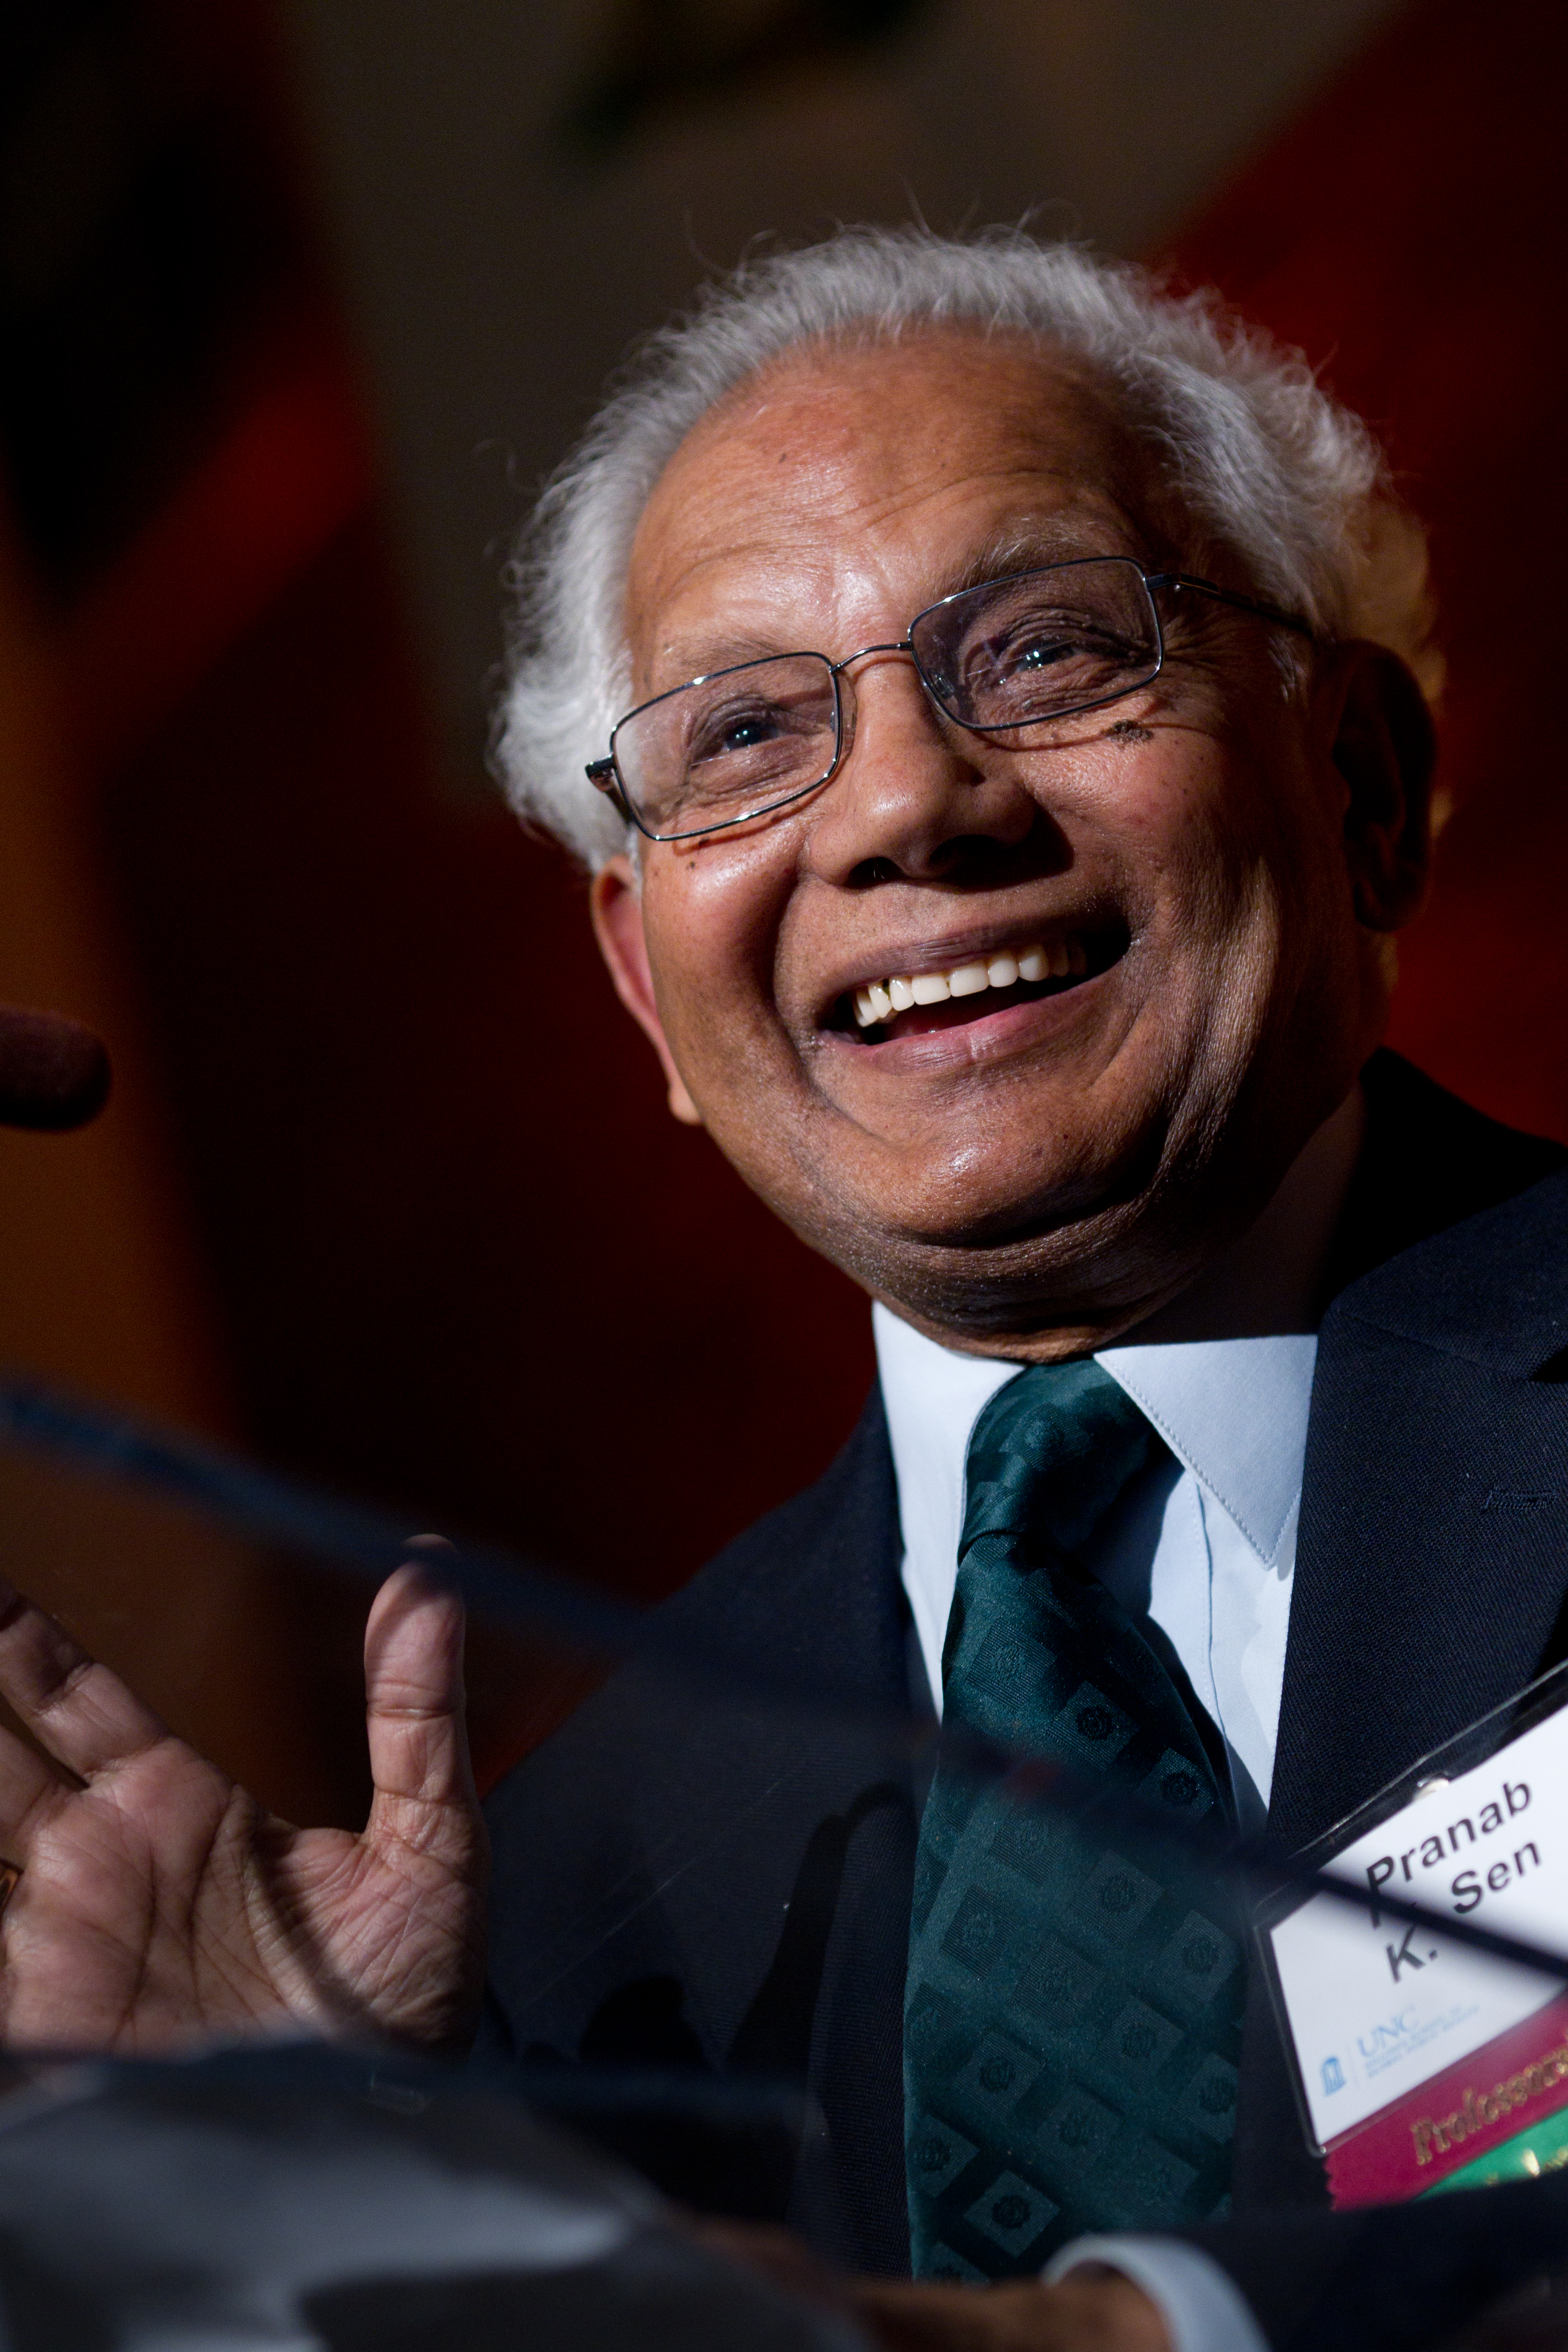
\includegraphics[width=0.45\linewidth]{rysunki/sen_now.jpg}
\caption{Prof. dr. Pranab Kumar Sen, autor Tom Fuldner, r. 2011}
\label{rys:Pranab_K_Sen}
\end{figure}

\section{Metoda Theil-Sen}
Metoda Theil-Sen, nazwana również estymatorem Theil-Sen, to technika dopasowywania prostej linii regresji na podstawie mediany nachyleń wszystkich linii przechodzących przez pary punktów istniejących w danym zbiorze.

Niech $x_i, x_j, \ldots, x_n$ oraz $y_i, y_j, \ldots, y_n$ będą niezależnymi punktami należącymi do zbioru liczb rzeczywistych.

Nachylenia wszystkich linii przechodzących przez pary punktów:

\[m_{ij} = \frac{y_j - y_i}{x_j - x_i}\]
Mediana nachyleń:
\[m = {mediana}\ \ m_{ij}\]
Obliczenie wyrazu wolnego (b) jako medianę wartości (yi - mxi):
\
\[b = {mediana}\ (y_i -mx_i)\]
Ostateczna linia regresji ma postać:
\[y=mx+b\]



\begin{figure}[h!]
\centering
\includegraphics[width=0.8\linewidth]{theil2.png}
\caption{Wykres metody Theil-Sen}
\label{fig:enter-label}
\end{figure}
Metoda ta jest szczególnie przydatna, gdy chcemy znaleźć linie ternu, ale występuje możliwość, że kilka nietypowych wartości zniekształci wynik.

Metoda Theil-Sen ma szerokie zastosowania w statystyce nieparametrycznej wymagającej założeń dotyczących rozkładu błędów, szerzej opisanych w artykule „Unbiasedness of the Theil–Sen estimator” z 2005 roku~\cite{wang2005}.

\section{Metoda najmniejszych kwadratów}

Metoda najmniejszych kwadratów ~\cite{linnik1962}~\cite{rand2010}(z angielskiego Method of Least Squares OLS) jest techniką stosowaną w statystyce, polegającą na dopasowaniu linii prostych (lub krzywych) do zbioru danych~\cite{bartoszewicz1989}~\cite{zieliński1990}. Jej celem jest wyznaczenie linii regresji, która najlepiej dopasuje się do danych punktów. Przedstawia się ją jako prostą y = ax + b, gdzie "a" to nachylenie, "b" to punkt przecięcia z osią y.

Dla zbioru danych $(x_1,y_1),(x_2,y_2)\ldots(x_n,y_n)$, szukana jest prosta $y=ax+b$, dla której suma kwadratów odchyleń między rzeczywistymi wartościami a wartościami przewidywanymi przez linię $y_i=ax_i+b$ była minimalna.

Suma z reszty kwadratów
\begin{equation*}
S(a,b) = \sum (y_i - (ax _i+b))^2
\end{equation*}


Aby znaleźć wartości dla, a i b, należy zminimalizować funkcję S(a,b). By to osiągnąć, należy zróżniczkować funkcję S względem, a i b, a następnie przyrównać te pochodne do zera.

Dla a:

\begin{equation*}
\frac{\partial S}{\partial a} = -2 \sum^n_{i=1} x_i (y_i - (ax _i+b))=0
\end{equation*}

Dla b:

\begin{equation*}
\frac{\partial S}{\partial b} = -2 \sum^n_{i=1} (y_i - (ax _i+b))=0
\end{equation*}

Metoda najmniejszych kwadratów  jest kluczowym narzędziem w analizie regresji, stosowanym w przeróżnych przypadkach. Dzięki efektywności obliczeniowej znajduje zastosowanie w takich dziedzinach jak analiza sygnałów, optymalizacja procesów technologicznych czy prognozowanie ekonomiczne.

Jednym z przykładów zastosowania tej metody jest artykuł z 2006 roku, w którym wykorzystano ją do identyfikacji oraz separacji składowych harmonicznych prądu obciążenia w aktywnych filtrach mocy, co umożliwiło skuteczną kompensację zakłóceń i poprawę jakości energii elektrycznej ~\cite{chudamani2006}. 


\begin{figure}[h!]
\centering
\includegraphics[width=0.77\linewidth]{kwadrat1.png}
\caption{Wykres metody najmniejszych kwadratów}
\label{rys:enter-label}
\end{figure}

\section{Porównanie metody}

Metoda Theil-Sen i metoda najmniejszych kwadratów to dwa podejścia do wyznaczania linii regresji.

\begin{figure}[h!]
\centering
\includegraphics[width=0.75\linewidth]{kwathe1.png}
\caption{Wykres obu metod}
\label{fig:enter-label}
\end{figure}
 
Metoda najmniejszych kwadratów minimalizuje sumę kwadratów odchyleń między przewidywanymi a rzeczywistymi wartościami.
Co sprawia, że jest szybsza, bardziej wydajna obliczeniowo oraz lepiej radzi sobie przy dużych zbiorach danych. Z kolei estymator Theil-Sen wyznacza nachylenie jako medianę nachyleń wyliczoną ze wszystkich możliwych par punktów, co czyni go dużo bardziej odpornym na wartości odstające. Fakt ten oznacza, że jest lepszą metodą w sytuacjach, gdzie istnieją dane o odstających wartościach i czas obliczeń nie jest istotny. Obie metody znajdują zastosowanie w analizie finansowej. W artykule z 2015 roku omówiono wykorzystanie metody najmniejszych kwadratów do prognozowania przyszłych wyników finansowych oraz przeprowadzono porównanie z metodą Theil-Sen. Analiza wykazała, że metoda Theil-Sen lepiej radzi sobie z wartościami odstającymi, zapewniając bardziej wiarygodne wyniki w porównaniu do metody najmniejszych kwadratów~\cite{james2015}.
%\input{tekst/donapisania}

\chapter{Porównanie metod przy użyciu środowiska Python}
W celu obrazowego porównania obu metod należy przygotować program w języku Python, który zmierzy czas wykonywania obliczeń, wyznaczy współczynniki nachylenia i wyrazy wolny dla każdej z metod oraz przedstawi wyniki na wykresie~\cite{amit2021}~\cite{mark2022}~\cite{luciano2015}.


\section{Kod źródłowy Theil-Sen}

Program realizuje obliczenia za pomocą algorytmu Theil-Sen, wyznaczając współczynnik nachylenia i wyraz wolny. Następnie generuje wykres, na którym przedstawione są dane wejściowe oraz dopasowana do nich linia regresji, umożliwiając wizualną ocenę działania estymatora.

\begin{lstlisting}[language=Python,
caption={Program Theil-Sen},
label={lst:hellopy}]
import numpy as np
import matplotlib.pyplot as plt
from sklearn.metrics import mean_squared_error

\end{lstlisting}

Na listingu 1 importowane są potrzebne biblioteki: NumPy do operacji numerycznych, Matplotlib do tworzenia wykresów oraz mean\_squared\_error do obliczania błędu średniokwadratowego (MSE), który jest miarą stosowaną do oceny jakości dopasowania modelu do danych. 

\begin{lstlisting}[language=Python,
caption={Program Theil-Sen},
label={lst:hellopy}]
def mediana(tablica):
tablica_posortowana = np.sort(tablica)
dlugosc = len(tablica_posortowana)
if dlugosc % 2 == 0:
return (tablica_posortowana[dlugosc // 2 - 1] + tablica_posortowana[dlugosc // 2]) / 2.0
else:
return tablica_posortowana[dlugosc // 2]

\end{lstlisting}

Funkcja służy do obliczania mediany z tablicy. Na samym początku sortuje dane od najmniejszych do największych, wykorzystując funkcję np.sort(). Następnie zwraca wartości mediany. Jeśli zbiór elementów jest parzysty, funkcja zwraca średnią dwóch środkowych liczb, a jeśli jest nieparzysty, to środkową wartość.

\begin{lstlisting}[language=Python,
caption={Program Theil-Sen},
label={lst:hellopy}]

def regresja_theil_sen(x, y):
n = len(x)
nachylenia = []
wyrazy_wolne = []
\end{lstlisting}

Na Listing 3  zdefiniowana jest funkcja regresja\_theil\_sen, która implementuje estymator Theil-Sen. Funkcja rozpoczyna od obliczenia długości wektora x oraz inicjalizacji dwóch pustych list: nachylenia i wyrazy\_wolne. Listy te będą przechowywać odpowiednio wszystkie obliczone nachylenia i wyrazy wolne.

\begin{lstlisting}[language=Python,
caption={Program Theil-Sen},
label={lst:hellopy}]
for i in range(n):
    for j in range(i + 1, n):
        if x[i] != x[j]: 
        nachylenie = (y[j] - y[i]) / (x[j] - x[i])
        nachylenia.append(nachylenie)
 mediana_nachylenia = mediana(nachylenia)
\end{lstlisting}

Zostały zdefiniowane pętle for, w których obliczane są nachylenia każdej pary punktów (xi, xj) zgodnie ze wzorem regresji metodą Theil-Sena. Następnie, przy użyciu metody append(), obliczone wartości nachyleń są dodawane do listy. Po zakończeniu pętli, na podstawie zgromadzonych wartości, obliczana jest mediana nachyleń.

\begin{lstlisting}[language=Python,
caption={Program Theil-Sen},
label={lst:hellopy}]
for i in range(n):
    wyrazy_wolne.append(y[i] - mediana_nachylenia * x[i])
mediana_wyrazu = mediana(wyrazy_wolne)
wynik = {'nachylenie': mediana_nachylenia, 'wyraz_wolny': mediana_wyrazu}
    return wynik

\end{lstlisting}

Na tej samej zasadzie obliczany jest wyraz wolny. Zgromadzone wartości wyrazów wolnych są dodawane do listy, a następnie obliczana jest ich mediana. Na koniec zwracany jest wynik zawierający obliczone wartości nachylenia oraz wyrazu wolnego.

\begin{lstlisting}[language=Python,
caption={Program Theil-Sen},
label={lst:hellopy}]
x = np.random.randn(100, 1)
y = 3 * x.flatten() + 2 + np.random.randn(100) * 2
\end{lstlisting}

Ustawienie ziarna losowości zapewnia otrzymanie zawsze takiego samego punktu wyjścia, więc przy każdym uruchomieniu kodu generowane liczby będą identyczne. Co zapewni te same wyniki. Następnie stworzona zostaje tablica x zawierająca 100 losowych liczb w przedziale od 0 do 10 oraz tablica y, której każda z wartości jest wynikiem równania y = 3x + 2 z dodatkiem szumu (losowych odchyłek).

\begin{lstlisting}[language=Python,
caption={Program Theil-Sen},
label={lst:hellopy}]
wynik = regresja_theil_sen(x, y)  
y_przewidziane_theil_sen = przewidz(x, wynik)  
mse = mean_squared_error(y, y_przewidziane_theil_sen)

\end{lstlisting}

Zmienna wynik zawiera dopasowany model regresji Theil-Sen do danych wejściowych x i y. Na podstawie tego modelu przewidywane są wartości y dla każdego punktu x. Na koniec obliczany jest błąd średniokwadratowy (MSE), który ocenia jakość dopasowania modelu do rzeczywistych danych. Jest on wyrażony jako średnia kwadratów różnic między wartościami rzeczywistymi a wartościami przewidywanymi przez model.

\begin{lstlisting}[language=Python,
caption={Program Theil-Sen},
label={lst:hellopy}]
print("Metoda Theil-Sena:")
print(f"Nachylenie (wspolczynnik kierunkowy): {model_theil_sen.coef_[0]:.2f}")
print(f"Przesuniecie (punkt przeciecia z osia Y): {model_theil_sen.intercept_:.2f}")
print(f"Blad sredniokwadratowy (MSE): {mse:.2f}")

\end{lstlisting}

Kod wyświetla za pomocą funkcji print wartości współczynników regresji Theil-Sena, w tym nachylenie, przesunięcie oraz obliczony błąd średniokwadratowy (MSE). Wyniki są zaokrąglone do dwóch miejsc po przecinku.

\begin{lstlisting}[language=Python,
caption={Program Theil-Sen},
label={lst:hellopy}]

plt.figure(figsize=(10, 6))
plt.scatter(x, y, color='blue', label='Dane rzeczywiste', alpha=0.6)
plt.plot(x, y_pred, color='black', label='Regresja Theil-Sen', linewidth=2)
plt.xlabel('x')
plt.ylabel('y')
plt.title('Regresja metoda Theil-Sen')
plt.legend()
plt.grid(True)
plt.show()
\end{lstlisting}

W fragmencie kodu tworzony jest wykres, na którym przedstawiane są rzeczywiste dane, oraz linia regresji uzyskana za pomocą metody Theil-Sena. Rzeczywiste dane są reprezentowane przez niebieskie punkty, natomiast przewidywana linia regresji Theil-Sena jest zaznaczona czarną linią. Dodatkowo wykres zawiera opisy osi, tytuł oraz podziałkę, co ułatwia interpretację wyników.

\begin{figure}[h!]
\centering
\includegraphics[width=0.7\linewidth]{theil.png}
\caption{Wizualizacja metody Theil-Sen}
\label{rys:Wykres metody Theil-Sen}
\end{figure}

Po przeprowadzonych obliczeniach metodą Theil-Sen wyświetlany jest wynik nachylenia, wyrazu wolnego oraz błędu średniokwadratowego.

Nachylenie (współczynnik kierunkowy): 2.59

Przesunięcie (punkt przecięcia z osią Y): 2.13

Błąd średniokwadratowy (MSE): 3.81

\section{Kod źródłowy metody najmniejszych kwadratów}

Program realizuje obliczenia linii regresji metodą najmniejszych kwadratów (OLS), dopasowując ją tak, aby minimalizować różnice między danymi a modelem. Następnie generuje wykres, na którym przedstawione są punkty danych i dopasowana linia, co pozwala ocenić działanie metody.

\begin{lstlisting}[language=Python,
caption={Program metody najmniejszych kwadratów},
label={lst:hellopy}]
import numpy as np
import matplotlib.pyplot as plt
from sklearn.linear_model import LinearRegression
from sklearn.metrics import mean_squared_error

\end{lstlisting}

Na Listing 10 przedstawiono wykorzystanie modułu sklearn.linear\_model oraz klasy LinearRegression, która służy do przeprowadzenia regresji liniowej metodą najmniejszych kwadratów. Dodatkowo, do oceny jakości dopasowania modelu zastosowano błąd średniokwadratowy.
Wszystkie inne kroki w kodzie, takie jak dopasowanie modelu do danych, przewidywanie wartości czy wizualizacja wyników, pozostają bez zmian.

\begin{figure}[h!]
\centering
\includegraphics[width=0.7\linewidth]{kwadrat1.png}
\caption{Wizualizacja metody najmniejszych kwadratów}
\label{rys:enter-label}
\end{figure}
Po wykonaniu obliczeń metodą najmniejszych kwadratów wyznaczana jest wartości współczynnika nachylenia, wyrazu wolnego oraz  błędu średniokwadratowego.

Nachylenie (współczynnik kierunkowy): 2.78

Przesunięcie (punkt przecięcia z osią Y): 2.08

Błąd średniokwadratowy (MSE): 4.89






\section{Porównanie metod Thei-Sen i OLS}

\begin{lstlisting}[language=Python,
caption={Program dla obu metod},
label={lst:hellopy}]
import numpy as np
import matplotlib.pyplot as plt
from sklearn.linear_model import TheilSenRegressor
from sklearn.metrics import mean_squared_error
import time

\end{lstlisting}

W tym przypadku zostanie wykorzystana już  gotowa biblioteka Theil-Sen z dodaną biblioteką 'time', która będzie odpowiedzialna za mierzenie czasu, co pozwoli na sprawdzenie, która z metod jest szybsza.

\begin{lstlisting}[language=Python,
caption={Program dla obu metod},
label={lst:hellopy}]
num_outliers = 100
indices = np.random.choice(range(500), num_outliers, replace=False)
x[indices] = x[indices] + np.random.uniform(2, 5, (num_outliers, 1))
y[indices] = y[indices] + np.random.uniform(-10, 10, num_outliers)

\end{lstlisting}
Użyta tu komenda służy do wyboru losowych punktów odstających oraz zwiększenia wartości x dla punktów.

\begin{lstlisting}[language=Python,
caption={Program dla obu metod},
label={lst:hellopy}]
start_time_theil_sen = time.perf_counter()
model_theil_sen = TheilSenRegressor()
model_theil_sen.fit(x, y)
y_przewidziane_theil_sen = model_theil_sen.predict(X)
end_time_theil_sen = time.perf_counter()
time_theil_sen = end_time_theil_sen - start_time_theil_sen
\end{lstlisting}

Na listingu 13 dokonywany jest pomiar czasu trwania obliczeń dla metody  Theil-Sen. Proces ten polega na zainicjowaniu modelu regresji oraz dopasowaniu go do danych. Zapisujemy czas rozpoczęcia pomiaru, a następnie wykonujemy wszystkie operacje związane z dopasowaniem. Na końcu mierzymy czas zakończenia obliczeń, a różnica między tymi dwoma momentami daje czas trwania obliczeń dla metody.

\subsection{Porównanie wyników}

\begin{figure}[h!]
\centering
\includegraphics[width=0.7\linewidth]{THKW.png}
\caption{Wizualizacja obu metod}
\label{fig:enter-label}
\end{figure}

\begin{table}[!h]
\centering
\begin{tabular}{p{8 cm} |c|c}
& Theil-Sen & OLS\\\hline
Nachylenie (współczynnik kierunkowy) & 2.81 & 1.87\\\hline
Przesunięcie (współczynnik przesunięcia z osią Y) & 1.87 & 1.51\\\hline
Czas obliczeń [s] & 0.2806 & 0.0003\\\hline
Błąd średniokwadratowy (MSE) & 4.68 & 4.89\\\hline

\end{tabular}
\caption{\label{tab:zjawiska2}Porównanie wyników}
\end{table}

W tym przypadku celowo jest dodane dużo punktów oraz wartości odstającej, by lepiej zaobserwować różnicę w obu metodach. Z tabeli i wykresu można wysnuć wnioski, iż metoda Theil-Sen (linia czerwona) poprawniej dopasowała linię regresji do podanych punktów w porównaniu do metody najmniejszych kwadratów (czarna prosta). Za to w tej drugiej wynik udało się uzyskać w krótszym czasie. Co zgadza się z początkowymi założeniami odnośnie do obu metod~\cite{hristo2019}~\cite{james2015}.

Metoda Theil-Sena posiada szereg zalet, które czynią ją atrakcyjną alternatywą w stosunku do innych technik regresji, szczególnie w kontekście danych zawierających wartości odstające. Dzięki swojej odporności na wpływ punktów odstających metoda ta może zapewniać dokładniejsze wyniki w przypadkach, gdy tradycyjne metody, takie jak regresja najmniejszych kwadratów, mogą być podatne na zniekształcenia wynikające z takich anomalii. Z tego powodu implementacja estymatora Theil-Sena na mikrokontrolerze STM32 może okazać się korzystnym rozwiązaniem, szczególnie w aplikacjach, w których dane wejściowe charakteryzują się dużą zmiennością lub obecnością wartości odstających.

\chapter{Implementacja estymatora Theil-Sen w środowisku STM32}
Kody w STM32 stanowią główną część pracy. Pierwszy z nich, czyli plik main.c, odpowiada za konfigurację mikrokontrolera. Kolejne pliki, theil\_sen.c oraz theil\_sen.h, zawierają implementację samego algorytmu Theil-Sen i odpowiadają za jego działanie. Taki podział kodu pozwala na wyraźne rozgraniczenie funkcji związanych z obsługą mikrokontrolera od właściwej logiki obliczeniowej~\cite{UM1727}~\cite{ionescu2020}~\cite{jacko2019}.

\section{main.c}
Jest to główny plik odpowiadający za konfigurację mikrokontrolera oraz dostarczanie wyników~\cite{francuz2015}~\cite{prata2016}.

\lstinputlisting[language=C,
firstnumber=30,
firstline=30,
lastline=34,
caption=\lstname,
label={lst:Keccak}]{main.c}

Na listingu 14 "string.h" dodaje funkcje do pracy z ciągami znaków. "stdio.h" umożliwia korzystanie z funkcji wejścia/wyjścia, takich jak printf do wyświetlania informacji. "theil\_sen.h" wprowadza deklaracje funkcji związanych z algorytmem Theil-Sen.

\lstinputlisting[language=C,
firstnumber=42,
firstline=42,
lastline=44,
caption=\lstname,
label={lst:Keccak}]{main.c}

Ustawienie tablicy na maksymalną wartość równą 4095, czyli maksymalną wartość bitową mikrokontrolera.

\lstinputlisting[language=C,
firstnumber=53,
firstline=53,
lastline=61,
caption=\lstname,
label={lst:Keccak}]{main.c}

\lstinputlisting[language=C,
firstnumber=107,
firstline=107,
lastline=110,
caption=\lstname,
label={lst:Keccak}]{main.c}

Pierwsza funkcja ma za zadanie uruchomić przetwornik cyfrowo-analogowy (DAC) na kanale 1. Druga kalibruje przetwornik analogowo-cyfrowy (ADC) w trybie pojedynczego wejścia, co poprawia dokładność pomiarów.

\lstinputlisting[language=C,
firstnumber=113,
firstline=113,
lastline=131,
caption=\lstname,
label={lst:Keccak}]{main.c}

W pętli while znajduje się pętla for, która wykonuje się, dopóki zmienna "i" nie osiągnie wartości MAX\_VALUES, zdefiniowana wcześniej w kodzie jako 4095. Przy każdym wykonaniu pętli zmienna "i" jest inkrementowana, co powoduje zwiększenie wartości DAC o 1.

Pętla rozpoczyna się od komendy uruchamiającej ADC. Następnie program oczekuje na zakończenie przetwarzania sygnału analogowego przez ADC i ustawia odpowiednią wartość na DAC. Wynik z ADC jest odczytywany za pomocą funkcji HAL\_ADC\_GetValue i zapisywany do zmiennej value\_adc. Wartości y są równe wartościom value\_adc i zapisywane do tablicy.

Zmienne x są otrzymywane w analogiczny sposób, jednak dodatkowo dzielone są przez rezystancję "r" równą 330 Ω, zgodnie ze wzorem
I = U/R. Takie podejście pozwala uzyskać wyniki z precyzją do kilku miejsc po przecinku.
Aktualnie wartość value\_adc mieści się w zakresie od 0 do 4095. Dopiero po przeliczeniu na odpowiednią skalę (od 0 do 3,3 V) dane będą gotowe do prezentacji. Proces ten zostanie szczegółowo opisany w dalszej części pracy.

Aby lepiej zrozumieć cel i sposób działania, należy wyjaśnić, dlaczego używane są przetworniki DAC i ADC w tej implementacji. DAC pełni rolę wymuszenia, czyli generuje sygnał napięciowy sterujący, który jest podawany na wejście układu. ADC z kolei mierzy napięcie wynikowe, odpowiadające temu wymuszeniu.

Warto również wspomnieć o roli rezystora 330 Ω. Jego obecność ma na celu ograniczenie prądu w obwodzie, co zapobiega uszkodzeniu elementów, takich jak na przykład diody. W zależności od układu można tę wartość dowolnie zmieniać.

\lstinputlisting[language=C,
firstnumber=132,
firstline=132,
lastline=143,
caption=\lstname,
label={lst:Keccak}]{main.c}

Fragment kodu rozpoczyna się od obliczenia długości tablicy x, co realizowane jest przez podzielenie jej rozmiaru w bajtach przez rozmiar pojedynczego elementu. Następnie wywoływana jest funkcja TheilSen\_Estymator, która przyjmuje jako argumenty tablice x i y oraz ich długość. Funkcja zwraca strukturę WynikTheilSena, zawierającą wartości wyrazu wolnego i nachylenia.

Obliczone wartości są formatowane jako tekst za pomocą funkcji sprintf i zapisywane do zmiennej msg, która została zadeklarowana na początku programu. Ostatecznie wiadomość jest przesyłana przez UART za pomocą funkcji HAL\_UART\_Transmit, co umożliwia wyświetlenie wyników na urządzeniu zewnętrznym.

Aby zapewnić poprawne działanie i wyświetlanie wartości zmiennoprzecinkowych na urządzeniu zewnętrznym, konieczne było odpowiednie skonfigurowanie ustawień programu zgodnie z dokumentacją dotyczącą obsługi zmiennych typu float~\cite{UM2609}.

\lstinputlisting[language=C,
firstnumber=190,
firstline=190,
lastline=193,
caption=\lstname,
label={lst:Keccak}]{main.c}

Te funkcje służą do odbioru danych z mikrokontrolera przez UART za pomocą Tx i Rx.

\section{thil\_sen.c}
Plik realizuje procedurę obliczeniową opartą na algorytmie estymacji Theila-Sena, dedykowanym do wyznaczania parametrów regresji liniowej, takich jak współczynnik kierunkowy i wyraz wolny. Algorytm został zaimplementowany z uwzględnieniem optymalizacji pod kątem ograniczonych zasobów sprzętowych mikrokontrolera, co pozwala na efektywne przetwarzanie danych i uzyskiwanie wyników o wysokiej precyzji.

\lstinputlisting[language=C,
firstnumber=1,
firstline=1,
lastline=3,
caption=\lstname,
label={lst:Keccak}]{theil_sen.c}

Nagłówek theil\_sen.h włącza plik deklarujący funkcję i struktury związane z implementacją metody Theil-Sen. Stdlib.h jest to standardowa biblioteka C, która umożliwia sortowanie za pomocą funkcji qsort. Ostatnia biblioteka stddef.h pozwala na zdefiniowanie rozmiaru tablicy size\_t.

\lstinputlisting[language=C,
firstnumber=5,
firstline=5,
lastline=10,
caption=\lstname,
label={lst:Keccak}]{theil_sen.c}

Zostaje zdefiniowana wielkość MAX\_ELEMENTOW jako 4095.
Funkcja porownaj\_floaty porównuje dwie wartości. Jest używana jako funkcja pomocnicza w qsort do sortowania tablic. Parametry a, b są to wskaźniki typu float, za pomocą których obliczana jest różnica między wartościami.

\lstinputlisting[language=C,
firstnumber=12,
firstline=12,
lastline=19,
caption=\lstname,
label={lst:Keccak}]{theil_sen.c}

Funkcja mediana oblicza medianę wartości w tablicy liczb zmiennoprzecinkowych. Sortuje tablicę za pomocą qsort (korzysta z funkcji porownaj\_floaty). Mediana obliczana jest zgodnie z matematyczną definicją:
Jeśli liczba elementów jest parzysta, zwraca średnią z dwóch środkowych elementów.
Jeśli nieparzysta, zwraca środkowy element.

\lstinputlisting[language=C,
firstnumber=21,
firstline=21,
lastline=26,
caption=\lstname,
label={lst:Keccak}]{theil_sen.c}

Funkcja TheilSen\_Estymator oblicza estymację metodą Theila-Sena, przyjmując jako argumenty tablice współrzędnych x i y oraz ich długość. W jej wnętrzu deklarowane są tablice nachylenia i wyrazy\_wolne do przechowywania obliczonych wartości, a także zmienne pomocnicze indeks\_nachylen i indeks\_wyrazow, służące do określenia indeksu w dalszych obliczeniach.

\lstinputlisting[language=C,
firstnumber=28,
firstline=28,
lastline=32,
caption=\lstname,
label={lst:Keccak}]{theil_sen.c}

\lstinputlisting[language=C,
firstnumber=42,
firstline=42,
lastline=43,
caption=\lstname,
label={lst:Keccak}]{theil_sen.c}

Na listingu 25 i 26 obliczana jest mediana wartości przechowywanych w tablicy nachylenia, która zawiera obliczone nachylenia dla wszystkich par punktów. Funkcja mediana przyjmuje jako argumenty tablicę nachylenia oraz liczbę elementów w niej zapisanych (indeks\_nachylen) i zwraca wartość mediany, przypisywaną do zmiennej mediana\_nachylenia.

\lstinputlisting[language=C,
firstnumber=43,
firstline=43,
lastline=52,
caption=\lstname,
label={lst:Keccak}]{theil_sen.c}

Na listingu 27 obliczany jest wyraz wolny dla każdego punktu danych, wykorzystując wcześniej wyznaczoną medianę nachyleń. Dla każdego punktu (x[i], y[i]), obliczana jest wartość y[i] - {mediana nachylenia} x[i] , która zostaje zapisana w tablicy wyrazy\_wolne, o ile jej maksymalna pojemność nie zostanie przekroczona. Następnie wyznaczana jest mediana z tablicy wyrazy\_wolne, która reprezentuje wyraz wolny prostej regresji. Funkcja zwraca wynik w postaci struktury WynikTheilSena, zawierającej medianę nachyleń jako nachylenie prostej oraz medianę wyrazów wolnych jako punkt przecięcia z osią y.

\subsection{thil\_sen.h}

Jest to kod do implementacji metody Theila-Sena.

\lstinputlisting[language=C,
firstnumber=1,
firstline=1,
lastline=15,
caption=\lstname,
label={lst:Keccak}]{theil_sen.h}

Zawiera definicję struktury WynikTheilSena do przechowywania nachylenia i wyrazu wolnego linii regresji oraz deklarację funkcji TheilSen\_Estymator, która oblicza parametry regresji dla podanych danych x i y.

\section{Układ z rezystancyjnym dzielnikiem napięcia}

\begin{figure}[h!]
\centering
\includegraphics[width=0.8\linewidth]{rysunki/układ.jpeg}
\caption{Układ pomiarowy rezystory}
\label{rys:Układ pomiarowy}
\end{figure}

\subsection{Wykres i wynik}

Po wykonaniu programu uzyskano dane wyjściowe. Na podstawie tych danych wygenerowano wykres ilustrujący zależności wartości ADC/330 od wartości ADC (y od x). Na wykresie znajduje się linia regresji, wyznaczona metodą Theila-Sena. W celu poprawy czytelności wykresu liczba punktów została ograniczona do około 80, co stanowi reprezentatywną próbkę danych. Taka redukcja liczby punktów umożliwia lepszą interpretację wyników i wizualizację, bez utraty istotnych informacji.

\begin{figure}[h!]
\centering
\includegraphics[width=0.8\linewidth]{rysunki/ADC_I.jpg}
\caption{Wykres ADC/330 od ADC}
\label{rys:enter-label}
\end{figure}

Obliczenia metodą Theil-Sen nachylenia oraz punktu przecięcia z osią y zostały przeprowadzone dla wybranych punktów danych przy użyciu wcześniej opracowanego programu w środowisku Python. Z uwagi na przejrzystość wykresu obliczenia zostały przeprowadzone na ograniczonych wcześniej danych.

\begin{figure}[h!]
\centering
\includegraphics[width=0.7\linewidth]{rysunki/wynik_python.png}
\caption{Wynik ADC/330 od ADC w środowisku Python}
\label{rys:enter-label}
\end{figure}

Wyniki uzyskane z programu STM32CubeIDE są bardzo zbliżone do tych otrzymanych w Pythonie. Niewielkie różnice mogą wynikać z faktu, że tym pierwszym obliczenia są wykonywane na pełnej próbce danych, obejmującej 4096 punktów. W przeciwieństwie do tego, w wersji programu w Pythonie, obliczenia zostały przeprowadzone na ograniczonej liczbie punktów (około 80), co może wpływać na dokładność i precyzję uzyskanych wyników. Mimo tych drobnych rozbieżności wyniki pozostają zbliżone, co świadczy o poprawności obu analizy, z uwzględnieniem różnic w liczbie punktów danych użytych do obliczeń.

\begin{figure}[h!]
\centering
\includegraphics[width=0.9\linewidth]{rysunki/wynik_rez1.png}
\caption{Wynik ADC/330 od ADC}
\label{rys:enter-label}
\end{figure}

\subsection{Przeliczenie wartości}
Uzyskane dane są przedstawione w postaci wartości bitowych. Aby przeliczyć je na wartości napięcia wyrażone w [V] oraz prądu w [mA], należy zastosować poniższe zależności:

\[U = \frac{ADC}{4096}*3,3 [V]\]
\[I = \frac{ADC/330}{4096}*1000 [mA]\]
gdzie:

• 4096 to maksymalna wartość z przetwornika DAC w mikrokontrolerze, wynikająca z 12-bitowej rozdzielczości (zakres od 0 do 2$^{12}$ - 1),

• 3.3 V to maksymalne napięcie przetwornika,

• 1000 to zamiana z A na mA.

Widać, że charakterystyka jest liniowa, co zgadza się z teoretycznymi założeniami dla rezystorów.
\begin{figure}[h!]
\centering
\includegraphics[width=0.8\linewidth]{rysunki/U_I.jpg}
\caption{Wykres U od I}
\label{rys:enter-label}
\end{figure}

\section{Układ z diodą i rezystorem}

Celem tego fragmentu pracy jest zaprezentowanie układu testowego, który umożliwia ocenę poprawności działania implementacji metody Theil-Sen dla przebiegu nielinioweg.

\begin{figure}[h!]
\centering
\includegraphics[width=0.9\linewidth]{rysunki/Dioda.jpg}
\caption{Płytka PCB}
\label{rys:enter-label}
\end{figure}

\subsection{Wykres i wynik}

W przeprowadzonym eksperymencie stworzono wykres porównujący sygnał odebrany przez przetwornik analogowo-cyfrowy (ADC) z sygnałem zadanym, generowanym przez przetwornik cyfrowo-analogowy (DAC). Na podstawie otrzymanych danych stworzono wykres, który pozwala wizualnie ocenić, czy układ działa zgodnie z założeniami projektowymi oraz, czy przetwarzanie sygnałów przebiega poprawnie. Analiza wykresu umożliwia szybkie wykrycie ewentualnych błędów w działaniu układu oraz ocenę jakości pomiarów.

\begin{figure}[h!]
\centering
\includegraphics[width=0.85\linewidth]{wykres_python_dioda.png}
\caption{Wykres ADC od DAC}
\label{rys:enter-label}
\end{figure}

Na wykresie przedstawiono trzy estymacje regresji liniowej dla różnych zakresów danych. Pierwsza estymacja (czerwona linia) została obliczona dla przedziału po x od 0 do 2500, czyli w zakresie, w którym charakterystyka diody pozostaje płaska. Druga estymacja (niebieska linia) obejmuje zakres od 2200 do 4095, gdzie charakterystyka diody liniowo rośnie. Zakresy te celowo nałożono na siebie, co umożliwia wyznaczenie ich punktu przecięcia.

Dodatkowo można zauważyć, że wykres jest zgodny z teoretyczną charakterystyką diody, co potwierdza poprawność zarówno układu, jak i zastosowanej metody. Otrzymane dane są wiarygodne, a układ działa zgodnie z oczekiwaniami.

\begin{figure}[h!]
\centering
\includegraphics[width=0.7\linewidth]{python_dioda.png}
\caption{Wyniki ADC od DAC w środowisku Python}
\label{rys:enter-label}
\end{figure}

Podobnie jak w poprzednim przypadku, wybrano reprezentatywną próbkę danych, składającą się z około 80 punktów pomiarowych. Na podstawie tych danych, przy użyciu algorytmu zaimplementowanego we wcześniejszej części pracy w środowisku Python, obliczono wartości nachylenia oraz wyrazu wolnego.

Wyraz wolny i nachylenie w przypadku pierwszej regresji (linia czerwona) wynoszą 0, co jest zgodne z założeniami. Charakterystyka diody w tym zakresie pozostaje płaska, co oznacza brak obserwowalnego wzrostu. Druga część analizy obejmuje przedział od 2200 do 4095, w którym charakterystyka diody rośnie liniowo. Dodatkowo wyznaczono punkt przecięcia prostych, co umożliwia określenie napięcia progowego diody U\(_f\).



Aby osiągnąć też ten efekt również w środowisku STM32, niezbędne będzie dokonanie drobnych modyfikacji w pliku theil\_sen.c. Zmiany te umożliwią uwzględnienie podzielnie zakresu na dwie części. 


\lstinputlisting[language=C,
firstnumber=5,
firstline=5,
lastline=5,
caption=\lstname,
label={lst:Keccak}]{theil_sen_PCB.c}


W pierwszej kolejności dokonana zostanie zamiana wartości, przyjmując maksymalną liczbę elementów równą 2500. Oznacza to, że program uwzględni jedynie wartości do 2500, czyli zakres, w którym charakterystyka diody pozostaje płaska i nie wykazuje wzrostu.

\begin{figure}[h!]
\centering
\includegraphics[width=0.9\linewidth]{0-2500.png}
\caption{Wyniki ADC od DAC dla wartości od 0 do 2500}
\label{rys:enter-label}
\end{figure}
 
Wyniki uzyskane w środowisku STM32 są zgodne z danymi otrzymanymi w środowisku Pythona, co potwierdza, że implementacja algorytmu została przeprowadzona poprawnie. 




W drugim zakresie, obejmującym przedział od 2200 do 4095, wartość MAX\_ELEMENTÓW zostaje przywrócona do 4095. 


\lstinputlisting[language=C,
firstnumber=29,
firstline=29,
lastline=30,
caption=\lstname,
label={lst:Keccak}]{theil_sen_PCB.c}

\lstinputlisting[language=C,
firstnumber=44,
firstline=44,
lastline=44,
caption=\lstname,
label={lst:Keccak}]{theil_sen_PCB.c}

Na listingu 30 i 31 początkowa wartość zmiennej “i” została ustawiona na 2200, co powoduje, że obliczenia będą przeprowadzane w zakresie od 2200 do 4095.


\begin{figure}[h!]
\centering
\includegraphics[width=0.9\linewidth]{rysunki/2200-4096.png}
\caption{Wyniki ADC od DAC dla wartości od 2200 do 4095}
\label{rys:enter-label}
\end{figure}


Jak widać, nachylenie jest bliskie 0,85, a punkt przecięcia będzie równy około -1840. W obu przypadkach otrzymane wyniki są zbliżone, co świadczy o zgodności implementacji oraz poprawności działania zarówno wersji kodu uruchomionej na mikrokontrolerze STM32, jak i tej działającej w środowisku Pythona. Taka zgodność wyników sugeruje, że proces obliczeniowy został przeprowadzony prawidłowo, a algorytm działa zgodnie z oczekiwaniami.




\section{Napotkane problemy}

Podczas implementacji kodu ograniczona pamięć mikrokontrolera uniemożliwiła przeprowadzenie najdokładniejszych z możliwych obliczeń.

Dla równania:
x[i] = value\_adc / r;

Wynik dzielenia value\_adc przez rezystancję równą 330 jest zaokrąglany do całkowitych wartości w zakresie od 0 do 7, co obniża precyzję obliczeń.

Aby zwiększyć dokładność, można zmodyfikować działanie, dzieląc przez liczbę zmiennoprzecinkową:
r = 330.0;

W tym przypadku uzyskiwana jest dokładność nawet do 11 miejsc po przecinku, np. x[1] = 0.00606060587. Jednak w kodzie theil\_sen.c występują wartości typu float, które mają precyzję do 8 miejsc po przecinku, co oznacza, że nie są wystarczające do dalszego przetwarzania danych, zwłaszcza że metoda wymaga bardziej złożonych obliczeń, generujących jeszcze większą liczbę cyfr po przecinku.

Logicznym rozwiązaniem tego problem byłoby zamiana wartości na typ double, który oferuje precyzję do 16 miejsc po przecinku. Niestety, ograniczona pamięć mikrokontrolera nie pozwala na przetwarzanie danych o tak dużej precyzji.

Ostatecznie precyzja oferowana przez typ float jest wystarczająca do realizacji dokładnych obliczeń w ramach bieżącego zastosowania. Jednak pozostawia to pole do dalszego rozwoju i ulepszania tego rozwiązania.


\chapter{Podsumowanie}
\label{ch:podsumowanie}
Niniejsza praca dotyczy implementacji estymatora Theil-Sen na mikrokontrolerze STM32, będącego metodą obliczania linii regresji odporną na wartości odstające. Kluczową zaletą tej metody jest jej niezawodność w przypadku danych pomiarowych, które mogą być zakłócone lub zniekształcone przez szum, co jest częstym zjawiskiem w pomiarach opartych na czujnikach. Dodatkowo estymator Theil-Sen został porównany z klasyczną metodą najmniejszych kwadratów, aby uwypuklić jego wady i zalety oraz zidentyfikować odpowiednie obszary jego zastosowań.
 

Przegląd literatury wskazuje, że metoda Theila-Sena cieszy się dużym zainteresowaniem w różnych dziedzinach analizy danych. W prognozowaniu cen Bitcoina, gdzie występuje wysoka zmienność, wykazuje ona większą odporność na wartości odstające w porównaniu do innych metod, co czyni ją bardziej efektywną w warunkach szybko zmieniającego się rynku~\cite{bitcoin2021}. Z kolei w artykule z 2024 roku estymator Theil-Sen został zastosowany w analizie danych hydrologicznych i atmosferycznych, gdzie wykazał lepszą skuteczność niż metoda najmniejszych kwadratów~\cite{zahra2024}. Szczególnie wyróżniał się odpornością na wartości odstające, zapewniając bardziej wiarygodne wyniki. Dodatkowo charakteryzował się mniejszym błędem obliczeniowym w porównaniu do innych metod regresyjnych.

 
Przeprowadzone w pracy testy potwierdzają, że estymator Theil-Sen jest lepszym wyborem do zadań, gdzie występują skrajne odchylenia w danych, podczas gdy klasyczna metoda najmniejszych kwadratów może prowadzić do zniekształconych wyników, co jest zgodne z obecnym stanem wiedzy. Krytyczna analiza wyników wskazuje, że wybór metody zależy od charakterystyki danych wejściowych oraz wymaganej odporności na błędy pomiarowe.

W pracy zaimplementowano estymator Theil-Sen w języku C z użyciem środowiska STM32CubeIDE oraz zaprojektowano układ pomiarowy z płytką PCB, co pozwoliło na przeprowadzenie testów w realnych warunkach. Testy te wykazały, że mimo ograniczonych zasobów mikrokontrolera STM32, możliwe jest skuteczne realizowanie zaawansowanych algorytmów statystycznych. Wartością dodaną projektu jest wykazanie, że nawet systemy wbudowane, o ograniczonej pamięci i mocy obliczeniowej, mogą być używane do realizacji zaawansowanych algorytmów, co wpisuje się w aktualne kierunki rozwoju technologii.

Podsumowując, celem pracy było opracowanie i implementacja algorytmu Theil-Sen w środowisku STM32CubeIDE, co zostało osiągnięte. Implementacja została przeprowadzona poprawnie, algorytm działa zgodnie z założeniami, a wyniki testów potwierdzają jego efektywność. Ponadto, praca wykazała użyteczność estymatora Theil-Sen w systemach wbudowanych, szczególnie w zastosowaniach wymagających analizy danych z płytek PCB. Mimo pewnych ograniczeń związanych z pamięcią i mocą obliczeniową udało się uzyskać wyniki o wysokiej jakości, co dowodzi, że metoda ta jest użytecznym narzędziem w takich systemach.
Cel pracy został osiągnięty, a założenia dotyczące porównania metod, implementacji oraz analizy wyników zostały zrealizowane. W przyszłości warto rozważyć dalszą optymalizację algorytmu oraz rozszerzenie implementacji o dodatkowe metody statystyczne. 


    % Bibliografia - musi być
    % Bibliography - must exist
    \bibliografia

    % Strony końcowe - można zakomentować, jeśli zbędne
    % Additional pages - comment out if not needed
    
   
    % Spis rysunków
    
    \listoffigures

  
\end{document}
%%%%%%%%%%%%%%%%%%%%%%%%%%%%%%%%%%%%%%%%%%%%%%%%%%%%%%%%%%%%%%%%%%%%%%%%%%%

